\documentclass[Main]{subfiles}

\begin{document}		
	

\chapter{Projektbeskrivelse}

Projektet er skrevet ud fra projektets kravspecifikaiton\cite{Kravspec}.
En bruger skal have mulighed for, at styre en drone af type Cyclone fra AeroQuad\cite{AQ-store}, vha. en fjernbetjening der udvikles specielt dertil, illustreret på Figur \ref{Fig:Aktor-oversigt}.

\begin{figure}[H]
\centering
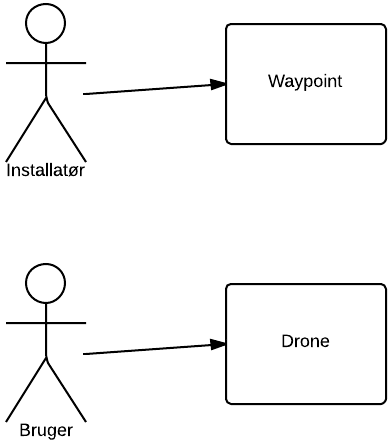
\includegraphics[scale=0.5]{AktQrDiagram}
\caption{Aktør-kontekst diagram}
\label{Fig:Aktor-oversigt}
\end{figure}

Brugeren kan styre dronen til at gøre følgende: Lette, lande, flyve frem, dreje til højre og venstre, øg og mindske rotationshastigheden, og hvis det skulle blive nødvendigt slukke for motorerne.

Foruden dette er dronen udstyret med 3 sonarsensorer, som kan registrere om der er forhindringer foran den og ud mod siderne.
Såfremt én af disse registrerer en forhindring, vil drone selv forsøge at flyve udenom forhindringen.
Til sidst er der også implementeret en sikkerhedsmekanisme, der vil standse motorerne hvis dronens propeller bliver beskadiget.













\end{document}	